This work was presented at the European Congress on Digital Pathology 2019 and published as part of its proceedings ~\citep{carse2019active}.



\section{Introduction}
\label{sec:active_introduction}
\subsection{Active Learning for Medical Image Analysis}
\label{subsec:active_for_medical_image_analysis}
Active learning is a type of machine learning that hypothesises that having a learning algorithm select the data that is used during training can reduce the amount of data needed for training~\citep{settles2009active}. Active learning is used within modern applications to reduce the quantity of data that needs to be annotated by selecting unannotated data to be annotated and added to the dataset used to train the model. Limiting the amount of data annotations needed can reduce annotation costs (which can be expensive when dealing with specialised data such as histopathology) and computation costs as the models can be trained with fewer data. In a pool-based scenario, the learning algorithm has access to a large pool of unannotated data. Over multiple iterations, the learning algorithm selects the most beneficial data from the pool to be annotated and added the training dataset, as shown in Figure~\ref{fig:pool_based_active_learning}. One of the main advantages of pool-based active machine learning for medical image analysis is its ability to reduce the amount of human labour required. Medical image analysis often involves manual annotation, which can be time-consuming and labour-intensive. By using pool-based active learning, the burden of annotation is greatly reduced, as the algorithm can identify the most informative samples and prioritise them for labelling.

Active learning algorithms utilise query strategies to select data for annotation. While some popular query strategies, such as uncertainty sampling, have been demonstrated to be effective on deep learning algorithms~\citep{gal2017deep}, the unique feature-representation learning process of deep learning algorithms can present challenges. Specifically, the selection of only difficult examples for training can lead to a lower-quality model due to the resulting features not being representative of the entire data distribution. This issue is illustrated by \cite{pop2018deep}, who demonstrate the occurrence of mode collapse when using a Bayesian uncertainty query strategy to train a CNN. To address these challenges, batch-aware query strategies that make use of clustering methods have been shown to be effective in deep learning environments~\citep{sener2017active, zhdanov2019diverse, kirsch2019batchbald}. These strategies optimise the selection of batches of images for annotation rather than individual data points.

\subsection{Deep Active Learning for Digital Pathology}
\label{subsec:active_deep_learning}
To save computation time, it is common practice in digital pathology to use patches from whole slide images when applying machine learning algorithms. These patches can be efficiently processed by deep learning algorithms like CNNs, and do not require the entire slide image to be annotated. However, using patch-based methods with patches for tasks such as nuclei detection and classification can be problematic when using active learning to query for annotation. This is because patches are more time-consuming and labour-intensive to annotate, and may lack sufficient spatial context for accurate annotation, even for expert pathologists.

To improve annotation efficiency and reduce costs, this chapter proposes a modified active learning framework to improve annotator throughput by selecting large regions of whole-slide images to be annotated rather than annotating individual nuclei patches. This modified framework was tested using various active learning query strategies on a nuclei detection and classification task using the CRCHistoPhenotypes dataset~\citep{sirinukunwattana2016locality}.



\section{Review of Active Learning for Medical Images}
\label{sec:active_review}
In recent years, active learning has undergone significant development in various areas, including query strategies for deep learning algorithms, techniques to reduce annotator workload, and application to medical image analysis tasks. This section provides an overview of key contributions in these domains that inform the present chapter's contribution.

\subsection{Pool-Based Active Learning Query Strategies}
\label{subsec:active_pool_based}
In pool-based active learning, a large pool of unannotated data and a small set of labelled data are utilised~\citep{settles2009active}. Query strategies are employed to identify the most useful unannotated data for annotation and incorporation into the learning algorithm (Figure \ref{fig:pool_based_active_learning}). This approach is particularly relevant in the context of medical image analysis, given the abundance of such data that is often collected and stored, but only a limited portion of which has been thoroughly annotated for use in machine learning applications. This review focuses on query strategies for pool-based active learning in both traditional and deep machine learning algorithms.

\subsubsection{Traditional Machine Learning Query Strategies}
As the focus of this chapter is limited to deep learning algorithms, only a brief review of pool-based active learning query strategies for traditional machine learning approaches will be performed.

\textbf{Uncertainty sampling} is a query strategy in which the learning algorithm focuses on data points it is most uncertain about to improve model performance~\citep{lewis1995sequential}. Uncertainty can be measured using techniques such as entropy or distance to the decision boundary. It allows the algorithm to selectively request labels for the most informative data points, leading to more efficient and effective learning. 

\textbf{Query by committee} is a query strategy in which a committee of multiple classifiers make predictions on unlabelled data~\citep{seung1992query}. If their predictions are diverse or conflicting, the learning algorithm may request a label for that data point. Query by committee can help reduce overfitting and improve generalisation.

\textbf{Expected model change} is a query strategy in which the learning algorithm estimates the change in overall performance after labelling a particular data point and prioritises data points with the greatest expected impact~\citep{settles2007multiple}. This allows the algorithm to focus on data points most likely to improve performance.

\textbf{Expected error reduction} is a method in active learning in which the learning algorithm estimates the reduction in error rate after labelling a particular data point, and prioritises data points with the greatest expected impact~\citep{roy2001toward}. This allows the algorithm to focus on data points most likely to improve performance. 

\textbf{Variance reduction} is a method in active learning in which the learning algorithm prioritises data points that are expected to have the greatest impact on reducing the variance of the predictions~\citep{cohn1996active}. This can be achieved by calculating the variance of the predictions for a particular data point. 

\textbf{Density-weighted methods} for active learning involve selecting data samples based on the density of the samples in the feature space, to select samples that are underrepresented or less dense~\citep{settles2008analysis}. These samples are likely to be more informative and valuable for the model to learn from, which can improve its performance and generalisation. There are several ways to implement density-weighted methods, including using a density estimate or weighting samples based on their informativeness and density.

\subsubsection{Deep Learning Query Strategies}
The application of active learning to deep learning algorithms has been met with various challenges~\citep{ren2021survey}. One such challenge is the increased data requirements of deep learning models, as they must concurrently learn both representative features and a classifier. Additionally, deep neural networks often experience issues related to confidence calibration, which can hinder the effectiveness of uncertainty-based active learning approaches due to the unreliable nature of softmax predictions as a measure of certainty. Within the field of deep active learning, two main categories can be identified: scoring query strategies, which select data for annotation based on a particular metric, and batch-aware query strategies, which select the optimal batch of data for annotation.

\subsubsection{Scoring Query Strategies}
To address the need for more representative data annotations, \cite{wang2016cost} proposed the \textbf{Cost-Effective Active Learning (CEAL)} algorithm. This algorithm is an extension of the standard uncertainty-based active learning method, which selects data for annotation based on uncertainty in the model's prediction (epistemic uncertainty). CEAL integrates a process called pseudo-labelling~\citep{lee2013pseudo}, in which data with low uncertainty used their predicted labels to augment the annotated data, resulting in a more diverse training set that includes both difficult, uncertain samples that can aid in classifier improvement, as well as certain samples that contribute to the development of a more generalised feature representation. The name CEAL reflects the cost-effective nature of this active learning approach, as it allows for the incorporation of new annotations without the associated labelling costs. The effectiveness of CEAL was evaluated in comparison to supervised learning, random active learning, and Triple Criteria Active Learning (TCAL)~\citep{demir2014novel} on the Cross-Age Celebrity Dataset~\citep{chen2014cross}. The results showed that CEAL achieved convergence with supervised learning using only 60\% of the data, outperforming both TCAL and random query methods in terms of convergence speed.

\cite{gal2016dropout} demonstrated that deep learning models employing softmax activation functions are unable to capture model uncertainty. To address this limitation, they introduced a method for approximating Bayesian inference using dropout in deep CNNs. Specifically, they applied dropout to each weight layer in the CNN during both training and testing and used the sample variance of the resulting prediction feedforward, which was repeated $B$ times, to estimate the model uncertainty. This process is depicted in Equation (\ref{eq:bayesian_cnn}), where $w$ represents the learned weights, $x$ denotes the input, and $\widehat{y}(b)$ is the CNN output obtained with dropout patten $b$ applied to each layer.

\begin{equation}
	Var(f(x, w))\approx\frac{1}{B}\sum^B_{b=1}\left(\widehat{y}(b)-\frac{1}{B}\sum\widehat{y}(b)\right)^2
	\label{eq:bayesian_cnn}
\end{equation}

\cite{gal2017deep} used Bayesian CNNs to evaluate a variety of active learning query strategies, including max entropy of the Bayesian samples~\citep{shannon1948mathematical}, variation ratios as a measure of uncertainty across the Bayesian samples~\citep{freeman1965elementary}, mean standard deviation across the Bayesian samples~\citep{kampffmeyer2016semantic}, Bayesian active learning disagreement (BALD)~\citep{houlsby2011bayesian}, and random sampling. The results indicated that variation ratios performed the best, followed closely by BALD and max entropy, while mean standard deviation performed similarly to the random baseline. However, the authors noted that the variation ratios method did not generalise well to more complex datasets, such as the ISIC skin lesion dataset~\citep{gutman2016skin}. In contrast, the BALD acquisition method demonstrated improved performance on these other datasets, and the use of Bayesian CNNs overall resulted in a significant improvement in performance compared to max entropy.

The Deep-Fool active learning method, proposed by \cite{ducoffe2018adversarial}, employs a strategy based on margin theory for sampling unannotated data that is close to decision boundaries. This approach, which has been previously discussed in the literature~\citep{settles2009active}, leverages adversarial attacks to determine the distance of a given data point to a decision boundary by adding small perturbations to the input image and measuring the resulting change in prediction~\citep{kurakin2018adversarial}. The query strategy subsequently selects the data closest to the decision boundary to be labelled, adding the labelled data and its adversarial counterparts to the training set.  According to the authors, this method exhibits competitive performance compared to core set active learning, while also being significantly less computationally complex and more efficient.

\subsubsection{Batch-Aware Query Strategies}
\cite{sener2017active} observed that when using CNNs, selecting a single piece of data can be detrimental to the training process due to its minimal statistical impact. They concluded that an active learning algorithm working with a CNN should choose an optimal batch of data for annotation. To achieve this, they treated the problem as a core-set selection problem, in which a small subset of data is selected to be representative of the entire dataset. This problem is equivalent to a k-center problem~\citep{farahani2009facility}, in which a set of $n$ points is chosen to cover all remaining data points while minimising the radius from each data point, as illustrated in Figure~\ref{fig:core-set}.

\begin{figure}[h]
	\centering
	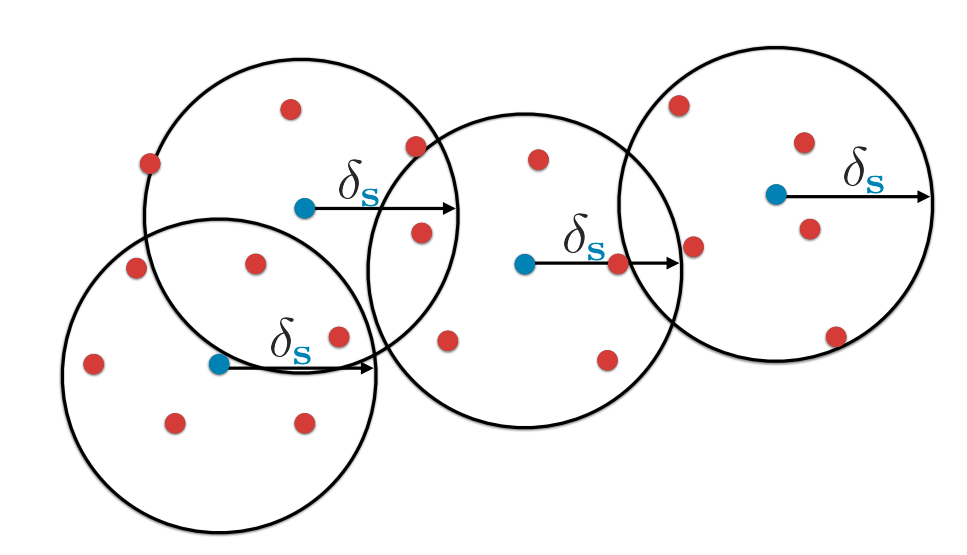
\includegraphics[width=0.75\textwidth]{images/core-set.png}
	\caption{A visual illustration of the core-sets query strategy, in which four points are selected that cover all other data points and minimise $\delta_s$~\citep{sener2017active}.}
	\label{fig:core-set}
\end{figure}

To compare their method to others, they conducted experiments with different selection methods, using Ladder Networks~\citep{rasmus2015semi} as a method for weakly supervised learning, as these can be trained on unlabelled data at each iteration. They discovered that for all selection algorithms tried weakly supervised learning significantly improved model performance. Results on the CIFAR 10 and CIFAR 100 datasets~\citep{krizhevsky2009learning} demonstrate that the core set method significantly outperformed the other methods evaluated.

\cite{kirsch2019batchbald} introduced BatchBALD, a batch-aware extension of BALD~\citep{gal2017deep}, which selects data points that exhibit high mutual information between model parameters and model output. To achieve this, the authors modify the definition of mutual information to incorporate both the general uncertainty of the model and the expected uncertainty for a specific set of model parameters. Submodularity is then utilised to identify the optimal set of data points that maximise mutual information. The authors demonstrate that BatchBALD outperforms BALD on multiple datasets, including MNIST~\citep{lecun1998gradient}, EMNIST~\citep{cohen2017emnist} and CINIC-10~\citep{darlow2018cinic}. However, the authors also acknowledge certain limitations of BatchBALD, including its reduced effectiveness on unbalanced datasets and the noise introduced using Monte Carlo dropout.

\cite{zhdanov2019diverse} introduced Diverse mini-batch active learning (DBAL), which combines uncertainty and diversity sampling to identify an optimal batch of data. The data is first encoded and then clustered using K-means, with data points closest to the centre of each cluster being selected. To incorporate uncertainty, weighted K-means is utilised, where each data point is assigned a weight based on an uncertainty function (in this case, margin-based uncertainty, which the authors found to be particularly effective). To improve computational efficiency, they pre-filter the unlabelled data points by uncertainty and only cluster the remaining data points. Demonstrated that DBAL outperforms other baselines on multiple datasets, including MNIST~\citep{lecun1998gradient} and CIFAR-10~\citep{krizhevsky2009learning}.

\subsection{Application of Active Learning for Medicine}
\label{subsec:active_applications}
Active learning has the potential to significantly reduce annotation costs in medical image analysis tasks, which has very expensive annotation costs~\citep{budd2021survey}. This is demonstrated by the PanNuke dataset \citep{gamper2019pannuke, gamper2020pannuke}, which was generated through a combination of machine learning algorithms trained on public datasets, and active learning methods to refine the annotations. Specifically, the authors used the algorithm to detect and classify nuclei in whole slide images, and then applied active learning techniques to measure the epistemic uncertainty and select the images for expert annotation. Through this approach, the authors were able to annotate 205,343 nuclei with 5 classification labels, with only 10\% of the data requiring manual annotation from pathologists. This serves as a compelling example of the utility of active learning in digital pathology, enabling the efficient construction of large and detailed datasets.

The survey of deep active learning for medical image analysis by \cite{budd2021survey}, covers a significant body of research. This research encompasses a diverse range of medical image analysis tasks, including but not limited to MRI segmentation~\citep{konyushkova2019geometry,zhao2019data}, skin lesion classification and segmentation~\citep{shi2019active, gorriz2017cost}, ultrasound classification~\cite{liu2020semi}, and histopathology whole slide image segmentation~\citep{folmsbee2021whole, jin2021reducing}. Despite this extensive research on active learning, the majority of the literature assumes that all annotations are equally costly, with little effort being made to account for the potential variations in annotation costs.

\subsection{Active Learning for Annotation Efficiency}
\label{subsec:active_annotation_efficiency}
Active learning is a widely researched methodology in the field of machine learning that emphasises the selective annotation of a subset of data, rather than annotating all available data, to improve the performance of machine learning algorithms while also reducing annotation costs. The traditional approach to active learning has been to assume that the costs of annotating all data are the same. However, recent research has indicated that this is not always the case in practice, with some data being more difficult to annotate than others~\citep{settles2008active}. In order to address this issue, various methods have been proposed to increase annotation efficiency, particularly in the context of deep learning algorithms. One such method is the cost-effective active learning approach tailored to multi-class semantic segmentation, known as CEREALS, which was proposed by \cite{mackowiak2018cereals}.

The Cost-Effective Region-based Active Learning for Semantic Segmentation (CEREALS) method reduces annotation costs by identifying informative image patches that have low annotation costs. The authors accomplished this by developing information maps and estimated annotation cost maps for each image, which were then fused to extract patches that maximise information while minimising annotation cost. The uncertainty for each pixel was calculated using vote entropy across Bayesian samples of the model, generated through the use of Monte Carlo dropout~\citep{gal2016dropout}. Annotation costs were approximated based on the number of clicks required to annotate the image. Evaluation of the CEREALS method on the Cityscapes dataset~\citep{cordts2016cityscapes} showed that it achieved high mean Intersection over Union (mIoU) scores while also requiring fewer annotator clicks when compared to other active learning methods. Building upon this approach, \cite{colling2020metabox+} proposed a similar method but modified the definition used to estimate the cost of annotating and demonstrated a reduced annotation cost compared to other algorithms that don’t take into account variable annotation costs.



\section{Annotator Efficient Active Learning for Histopathology}
\label{sec:active_annotator_efficient}
Annotation of medical images, particularly histopathology tasks, poses a significant challenge due to the cost and lack of expert annotators. For instance, tasks such as nuclei detection and classification necessitate annotators to meticulously select and categorise nuclei in whole slide images. A notable example of this can be observed in the annotation procedure for the CRCHistoPhenotypes dataset~\citep{sirinukunwattana2016locality}, in which annotators had to examine 500x500 pixel patches extracted from 100 H\&E slides (0.55 $\mu$m/pixel, equivalent to 20x optical magnification) and assign each nucleus a classification of epithelial, inflammatory, fibroblast, or miscellaneous. The annotations were collected by experienced pathologists and graduate students supervised by the same pathologists, highlighting the costly nature of such annotation efforts, given the financial requirements for expert annotators. This illustrates the potential for applying active learning methods that incorporate considerations of annotation cost.

\subsection{Region-Based Active Learning}
\label{subsec:active_region_based}
Patch-based approaches are widely used in digital pathology and medical image analysis. However, applying active learning to these methods can be laborious, particularly in systems that utilise small patches. These patches can be challenging to annotate in isolation, even when provided with spatial visual context. To address this, this chapter proposes a region-based approach that requests annotations over larger regions containing multiple small patches. Working with larger regions reduces the burden on the annotator and can increase the annotation collection throughput. This modification enables a learning algorithm to be trained on small patches, while treating the data as larger regions only when querying the unannotated data to be annotated (Figure~\ref{fig:nuclei_example}).

\begin{figure}[h]
	\centering
	\begin{subfigure}{0.3\textwidth}
		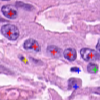
\includegraphics[width=\linewidth]{images/nuclei_example_1.png}
	\end{subfigure}
	\begin{subfigure}{0.3\textwidth}
		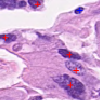
\includegraphics[width=\linewidth]{images/nuclei_example_2.png}
	\end{subfigure}
	\begin{subfigure}{0.3\textwidth}
		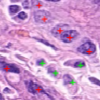
\includegraphics[width=\linewidth]{images/nuclei_example_3.png}
	\end{subfigure}
	\caption{Example regions that contain annotated nuclei to be extracted as patches and utilised for the purpose of training the model.}
	\label{fig:nuclei_example}
\end{figure}

The proposed query strategy involves a simple modification to an existing query strategy, as outlined in Algorithm~\ref{alg:regionbased}. In this algorithm, $S$ represents an existing query strategy, which is called at the end of each active learning iteration once a model has been trained on the current annotated data. The algorithm extracts all patches from each unannotated region and generates predictions for each patch, which are then averaged to obtain a prediction for the overall region. These region-level predictions can then be utilised within an active learning query strategy, such as entropy uncertainty sampling, to sample regions based on uncertainty values. This approach can also be applied to more complex query strategies, such as core-set sampling, by solving the K-centre problem for the region predictions rather than for individual data point feature representations.

\begin{algorithm}[h]
	\caption{Region-based active learning}
	\label{alg:regionbased}
	\SetKwInOut{Input}{Input}
	\SetKwInOut{Output}{Output}
	\SetKwProg{RegionQueryStrategy}{RegionQueryStrategy}{}{}
	\Input{
		$\theta :$ trained model,\\
		$\delta :$ prediction algorithm,\\
		$S :$ active learning query strategy,\\
		$U :$ set of unannotated data,\\
		$A :$ set of annotated data,\\
		$Y :$ empty set of region averages
	}
	\Output{
		$U' :$ updated set of unannotated data,\\
		$A' :$ updated set of annotated data
	}
	\RegionQueryStrategy{$\theta, \delta, S, U, A, Y$}
	{
		\ForEach{region $r$ in $U$}{
			$P \gets$ ExtractPatches($r$) \hfill extract patches from region\\
			$O \gets \delta(\theta, P)$ \hfill predictions on extracted patches\\
			$O' \gets$ Average($O$) \hfill average the patch predictions\\
			$Y \gets$ Append($Y, O'$) \hfill append region average to array\\
		}
		$n \gets S(Y)$ \hfill selects region from list\\
		$U' \gets$ Remove($U, n$) \hfill removes selection from unannotated set\\
		$A' \gets$ Append($A, n$) \hfill appends the selection to annotated set\\
		\Return{$U', A'$}
	}
\end{algorithm}



\section{Active Learning Experiments}
\label{sec:active_experiments}
This section describes the datasets, training parameters, experimental setup, and results for the experiments on nuclei classification using region-based active learning on whole slide image patches. The code and complete results for these experiments are available in the project GitHub repository\footnote{GitHub Repository: \url{github.com/jmcjacob/Patch-Active-Learning-Pathology}}.

\subsection{Dataset}
\label{subsec:active_dataset}
The publicly available CRCHistoPhenotypes dataset~\citep{sirinukunwattana2016locality} was used to evaluate the proposed region-based active learning approach, as it consists of a large number of annotated nuclei from large patches extracted from whole slide images, making it well-suited for this type of active learning. The dataset, which has also been utilised in multiple nuclei classification and detection studies, as well as active learning experiments~\citep{shao2018deep}, comprises 22,444 annotated nuclei from 100 500x500 pixel non-overlapping patches extracted from 10 H\&E whole-slide images of colorectal adenocarcinomas from 9 different patients. Each nucleus is annotated with its coordinates and corresponding classification (epithelial, inflammatory, fibroblast, or miscellaneous). The dataset includes 7,722 epithelial, 5,712 fibroblast, 6,971 inflammatory, and 2,039 miscellaneous annotated nuclei. 2,500 images were generated by dividing the patches into 100x100 pixel regions, from which each nucleus was extracted into a 30x30 patch for use in training the CNN model. During training, data augmentation was employed by randomly applying Gaussian blurring and horizontal and vertical flipping.

\begin{figure}[t!]
	\centering
	\begin{subfigure}{0.3\textwidth}
		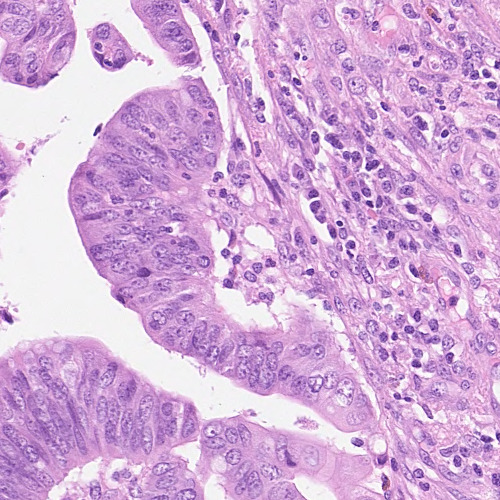
\includegraphics[width=\linewidth]{region1.jpg}
	\end{subfigure}
	\begin{subfigure}{0.3\textwidth}
		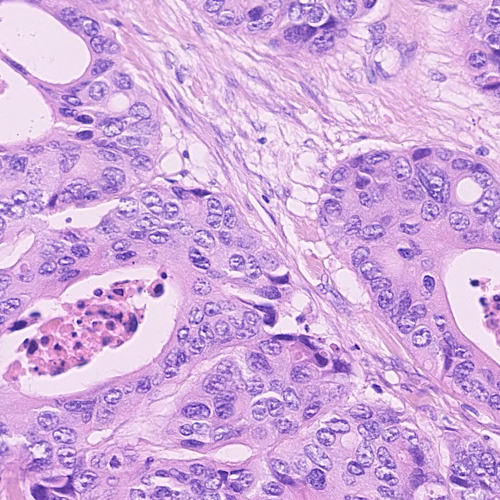
\includegraphics[width=\linewidth]{region2.jpg}
	\end{subfigure}
	\begin{subfigure}{0.3\textwidth}
		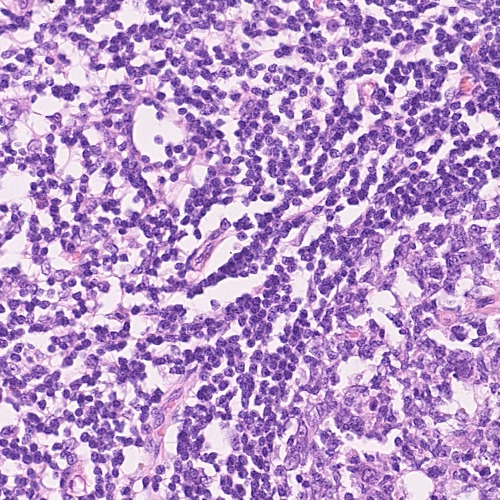
\includegraphics[width=\linewidth]{region3.jpg}
	\end{subfigure}
	\caption{Three example images from the CRCHistoPhenotypes dataset~\cite{sirinukunwattana2016locality} are shown, each containing multiple nuclei that will be extracted into patches and augmented.}
	\label{fig:region_example}
\end{figure}

\subsection{Training Parameters}
\label{subsec:active_training}
This experiment employed a CNN inspired by the architecture used in the nuclei classification benchmark for the CRCHistoPhenotypes dataset~\citep{sirinukunwattana2016locality}. The network consisted of two convolutional layers, the first with 36 4x4 filters and the second with 48 3x3 filters, each followed by a 2x2 max pooling layer. The convolutional layers were followed by two fully connected layers with 1200 and 512 neurons, respectively. This architecture is summarised in Table~\ref{tab:active_learning_cnn}. Each hidden layer utilised Rectified Linear Unit (ReLU) activation functions, while the fully connected layers employed dropout regularisation~\citep{srivastava2014dropout} with a drop rate of 0.5. Dropout was utilised during training to enable the use of Monte Carlo sampling after training.

\begin{table}[h]
	\caption{The Convolutional Neural Network architecture employed for nuclei classification in the region-based active learning experiments.}
	\label{tab:active_learning_cnn}
	\centering
	\begin{tabular}{|c|c|c}
		\hline
		Type & \begin{tabular}[c]{@{}c@{}}Filter\\ Dimensions\end{tabular} & \multicolumn{1}{c|}{\begin{tabular}[c]{@{}c@{}}Input/Output\\ Dimensions\end{tabular}} \\ \hline
		Input &  & \multicolumn{1}{c|}{30 x 30 x 3} \\ \hline
		Convolutional & 4 x 4 x 1 x 36 & \multicolumn{1}{c|}{26 x 26 x 36} \\ \hline
		Max Pooling & 2 x 2 & \multicolumn{1}{c|}{12 x 12 x 36} \\ \hline
		Convolutional & 3 x 3 x 36 x 48 & \multicolumn{1}{c|}{10 x 10 x 48} \\ \hline
		Max Pooling & 2 x 2 & \multicolumn{1}{c|}{5 x 5 x 48} \\ \hline
		Fully Connected & 5 x 5 x 48 x 1200 & \multicolumn{1}{c|}{1 x 1200} \\ \hline
		Fully Connected & 1 x 1 x 512 x 512 & \multicolumn{1}{c|}{1 x 512} \\ \hline
		Output & 1 x 1 x 512 x 4 & \multicolumn{1}{c|}{1 x 4} \\ \hline
	\end{tabular}

\end{table}

During the active learning process, the training environment is continuously evolving as the training data is incrementally expanded. To accommodate this dynamic situation, the Adadelta adaptive gradient descent algorithm~\citep{zeiler2012adadelta} was chosen, as it does not require manual tuning of the learning rate as it adjusts automatically to the gradients of the model. To prevent overfitting to the constantly changing training data, which may be limited in size, early stopping was employed. The approach proposed by \cite{prechelt2012early} compares the generalisation loss and training progression until a specified threshold of $\frac{GL(t)}{P_k(t)} > \alpha$ is reached. The generalisation loss (Equation \ref{eq:generalization_loss}) is calculated by comparing the validation loss at each epoch $L_{val}(t)$ to the minimum validation loss across all epochs, while the training progression (Equation \ref{eq:training_progression}) is calculated by analysing the training losses $L_{tr}(t)$ over a batch of recent epochs of size $k$.

\begin{equation}
	GL(t) = 100 \cdot \left ( \frac{L_{va}(t)}{\underset{t'\leq t}{min}L_{va}(t')} - 1 \right )
	\label{eq:generalization_loss}
\end{equation}
\begin{equation}
	P_k(t) = 1000 \cdot \left ( \frac{\sum_{t'=t-k+1}^{t}L_{tr}(t')}{k \cdot min^{t}_{t'=t-k+1}L_{tr}(t')} - 1\right )
	\label{eq:training_progression}
\end{equation}

\subsection{Experiment Setup}
\label{subsec:active_experiments}
A series of experiments were conducted to evaluate the effectiveness of the proposed region-based active learning approach in conjunction with various query strategies. These strategies included several basic methods, which served as baselines, as well as deep learning-specific query algorithms. The baseline strategies included random querying, least confident uncertainty, margin uncertainty, and entropy uncertainty sampling. The deep learning-specific query strategies tested were K-Centre sampling (employing greedy approximation), core-set sampling~\citep{sener2017active}, and BALD using Monte Carlo dropout~\citep{gal2017deep}. These methods were selected due to their state-of-the-art status in the field of deep active learning. 

In each experiment, all available data was initially treated as unannotated, and then two randomly selected regions were annotated to form an initial training dataset. During each active learning iteration, two additional regions were chosen from the pool of unannotated regions and added to the training dataset. A randomly initialised model (using uniform Xavier initialisation, as proposed by \cite{glorot2010understanding}) was then trained on the updated dataset. This process was repeated for 50 active learning iterations, resulting in a final training set of 102 regions out of 2,500 in each experiment. To account for random variations, each experimental condition was run five times, with different seeds used to generate random elements such as model weight initialisation and initial annotated patches.

\subsection{Results}
\label{subsec:active_results}
The performance of the various query strategies was assessed by evaluating the trained models on a fixed test set after each active learning iteration. Table~\ref{tab:query_results} presents the mean test accuracy and cross-entropy loss over five runs, after 50 iterations, for each of the query strategies. As shown, only the K-Centre sampling approach yielded higher average accuracy than a random sampling baseline. The core-set sampling strategy produced results that were similar to those of the random sampling approach, while the other query strategies all performed worse.

\begin{table}[h]
	\centering
	\caption{Test results for each query strategy after 50 active iterations.}
	\label{tab:query_results}
	\resizebox{\textwidth}{!}{%
		\begin{tabular}{c|ccccccc}
			\begin{tabular}[c]{@{}c@{}}Query\\ Strategy\end{tabular} & Random & \begin{tabular}[c]{@{}c@{}}Least \\ Confident\end{tabular} & Margin & Entropy & K-Centre & Core-Set & BALD \\ \hline
			Accuracy & 58.25 & 48.92 & 45.84 & 32.37 & 61.41 & 57.33 & 48.23 \\
			\begin{tabular}[c]{@{}c@{}}Mean Class \\ Accuracy\end{tabular} & 53.50 & 47.36 & 42.40 & 41.07 & 54.39 & 52.50 & 46.14 \\
			Loss & 1.154 & 1.243 & 1.268 & 1.39 & 1.123 & 1.157 & 1.247
		\end{tabular}%
	}
\end{table}

Figures~\ref{fig:active_learning_accuracy}, \ref{fig:active_learning_mean_class_accuracy}, and \ref{fig:active_learning_loss} illustrate the test accuracy, mean class accuracy, and cross-entropy loss for models trained with annotated data selected using each of the query strategies after each active learning iteration, averaged over five runs. The figures also include the results for a model trained using all 1487 annotated training regions; a fully supervised CNN trained on the entire annotated dataset achieved an accuracy of 68.53\% and a cross-entropy loss of 1.111. In contrast, the model trained with the K-Centre query strategy achieved an accuracy of 61.41\% and a cross-entropy loss of 1.137, using only 7\% of the annotated data.

\begin{figure}
	\centering
	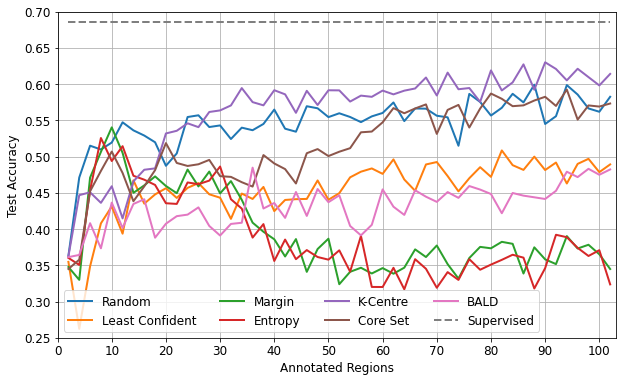
\includegraphics[width=\textwidth]{images/active_learning_accuracy.png}
	\caption{Average test accuracy of trained models using different amounts of annotated regions selected through various query strategies.}
	\label{fig:active_learning_accuracy}
\end{figure}

\begin{figure}
	\centering
	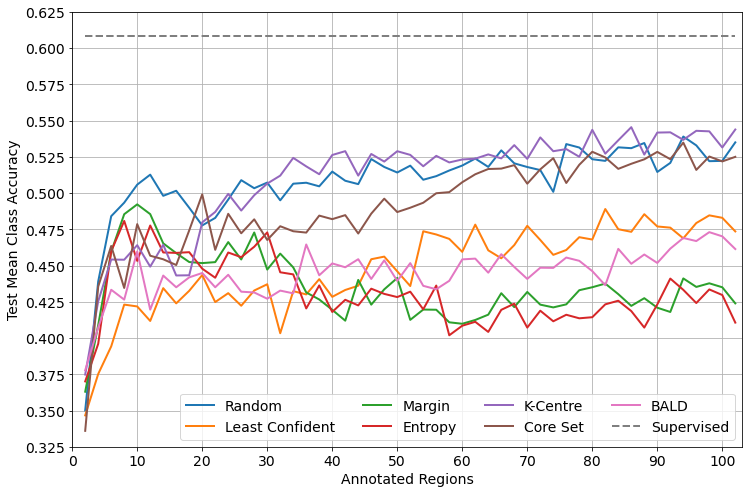
\includegraphics[width=\textwidth]{images/active_learning_mean_class_accuracy.png}
	\caption{Average test mean class accuracy of trained models using different amounts of annotated regions selected through various query strategies.}
	\label{fig:active_learning_mean_class_accuracy}
\end{figure}

\begin{figure}
	\centering
	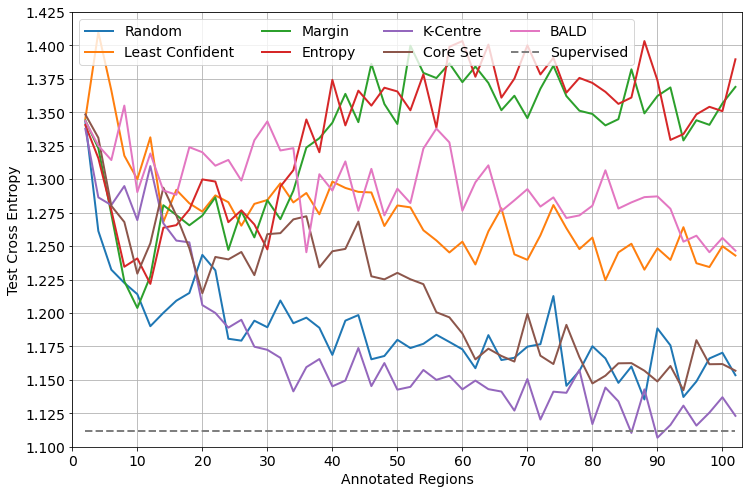
\includegraphics[width=\textwidth]{images/active_learning_loss.png}
	\caption{Average test loss of trained models using different amounts of annotated regions selected through various query strategies.}
	\label{fig:active_learning_loss}
\end{figure}



\section{Conclusion}
\label{sec:active_conclusion}
This chapter presents a method for mitigating the annotation burden in patch-based nuclei classification systems using deep active learning. The results reported in Section~\ref{subsec:active_results} indicate that traditional active learning approaches are less effective when applied to deep learning models, and that specialised active learning techniques for deep learning also fail to outperform random sampling baselines. This phenomenon, which has been previously noted in the literature on active learning for deep learning~\citep{ren2021survey}, highlights the need for more robust active learning methods in this domain.

Reducing the cost of annotating data is crucial for enabling the development of deep learning systems for digital pathology and medical image analysis, particularly for organisations with limited resources. While active learning holds promise as a means of addressing this challenge, further research is required to achieve meaningful improvements on tasks such as those presented in this chapter. This has motivated the investigation of unsupervised learning techniques as a complementary approach for leveraging unannotated data, potentially in conjunction with active learning.